\textbf{\Large Описание эксперимента}

В работе измеряется осмотическое давление водного раствора жёлтой кровяной соли $K_4 Fe (CN)_6$, при нескольких значениях концентрации и проверяется справедливость закона Вант-Гоффа.

Молекулы жёлтой кровяной соли при растворении диссоциируют:
$$
K_4 Fe (CN)_6 \rightarrow 4 K^+ + [Fe (CN)_6]^{4-}
$$

<<<<<<< Updated upstream
Ионы $K^+$ свободно проникают через используемую в работе перегородку и не создают осмотическое давление.

Начнём проводить измерения скорости движения мениска в капиляре от осмотического давления. Наблюдать прямой осмос при атмосферном давлении не удалось. За большой промежуток времени $\sim 5$ минут уровень мениска не изменился. При больших давлениях $>60$ делений манометра (1 деление $ = 245$ Па) наблюдается опускание уровня жидкости в капилляре с течением времени.

Измерим зависимость скорости опускания уровня жидкости в капилляре от давления при обратном осмосе.
=======
<<<<<<< Updated upstream
Ионы $K^+$ свободно проникают через используемую в работе перегородку и не создают осмотическое давление.
=======
Ионы $K^+$ свободно проникают через используемую в работе перегородку и не создают осмотическое давление.

Измерим зависимость скорости движения уровня жидкости в капилляре от давления при обратном осмосе.
>>>>>>> Stashed changes

\newpage

\large{\textbf{Концентрация $n = 0,3\%$}}

\begin{table}[H]
	\centering
	\begin{tabular}{c c c c}
		\begin{tabular}[t]{|c|c|}
\hline
$P$, дел & 0 \\
\hline
$t_{абс}$, с & $h$, мм \\ 
\hline
0,0 & 100,0 \\ 
85,0 & 105,0 \\ 
205,0 & 110,0 \\ 
335,0 & 115,0 \\ 
506,0 & 120,0 \\ 
\hline
\end{tabular}
		&
		\begin{tabular}[t]{|c|c|}
\hline
$P$, дел & 200 \\
\hline
$t_{абс}$, с & $h$, мм \\ 
\hline
0,0 & 200,0 \\ 
7,0 & 195,0 \\ 
14,0 & 190,0 \\ 
21,0 & 185,0 \\ 
28,0 & 180,0 \\ 
35,0 & 175,0 \\ 
\hline
\end{tabular}
		&
		\begin{tabular}[t]{|c|c|}
\hline
$P$, дел & 180 \\
\hline
$t_{абс}$, с & $h$, мм \\ 
\hline
0,0 & 200,0 \\ 
10,0 & 195,0 \\ 
20,0 & 190,0 \\ 
31,0 & 185,0 \\ 
42,0 & 180,0 \\ 
53,0 & 175,0 \\ 
\hline
\end{tabular}
		&
		\begin{tabular}[t]{|c|c|}
\hline
$n, \%$ & 0.3 \\
\hline
$P$, дел & 160 \\
\hline
$t_{абс}$, с & $h$, мм \\ 
\hline
0,0 & 200,0 \\ 
12,0 & 195,0 \\ 
24,0 & 190,0 \\ 
37,0 & 185,0 \\ 
50,0 & 180,0 \\ 
63,0 & 175,0 \\ 
\hline
\end{tabular}
	\end{tabular}
\end{table}

\begin{table}[H]
	\centering
	\begin{tabular}{c c c c}
		\begin{tabular}[t]{|c|c|}
\hline
$n, \%$ & 0.3 \\
\hline
$P$, дел & 140 \\
\hline
$t_{абс}$, с & $h$, мм \\ 
\hline
0,0 & 200,0 \\ 
17,0 & 195,0 \\ 
29,0 & 190,0 \\ 
47,0 & 185,0 \\ 
62,0 & 180,0 \\ 
78,0 & 175,0 \\ 
\hline
\end{tabular}
		&
		\begin{tabular}[t]{|c|c|}
\hline
$n, \%$ & 0.3 \\
\hline
$P$, дел & 120 \\
\hline
$t_{абс}$, с & $h$, мм \\ 
\hline
0,0 & 200,0 \\ 
18,0 & 195,0 \\ 
34,0 & 190,0 \\ 
53,0 & 185,0 \\ 
76,0 & 180,0 \\ 
94,0 & 175,0 \\ 
\hline
\end{tabular}
		&
		\begin{tabular}[t]{|c|c|}
\hline
$P$, дел & 100 \\
\hline
$t_{абс}$, с & $h$, мм \\ 
\hline
0,0 & 200,0 \\ 
27,0 & 195,0 \\ 
47,0 & 190,0 \\ 
75,0 & 185,0 \\ 
101,0 & 180,0 \\ 
126,0 & 175,0 \\ 
\hline
\end{tabular}
		&
		\begin{tabular}[t]{|c|c|}
\hline
$P$, дел & 80 \\
\hline
$t_{абс}$, с & $h$, мм \\ 
\hline
0,0 & 200,0 \\ 
38,0 & 195,0 \\ 
67,0 & 190,0 \\ 
106,0 & 185,0 \\ 
140,0 & 180,0 \\ 
179,0 & 175,0 \\ 
\hline
\end{tabular}
	\end{tabular}
\end{table}

\large{\textbf{Концентрация $n = 0,15\%$}}

\begin{table}[H]
	\centering
	\begin{tabular}{c c c c}
		\begin{tabular}[t]{|c|c|}
\hline
$P$, дел & 0 \\
\hline
$t_{абс}$, с & $h$, мм \\ 
\hline
0,0 & 101,0 \\ 
104,0 & 105,0 \\ 
270,0 & 110,0 \\ 
525,0 & 115,0 \\ 
\hline
\end{tabular}
		&
		\begin{tabular}[t]{|c|c|}
\hline
$P$, дел & 200 \\
\hline
$t_{абс}$, с & $h$, мм \\ 
\hline
0,0 & 200,0 \\ 
7,0 & 195,0 \\ 
14,0 & 190,0 \\ 
21,0 & 185,0 \\ 
28,0 & 180,0 \\ 
36,0 & 175,0 \\ 
\hline
\end{tabular}
		&
		\begin{tabular}[t]{|c|c|}
\hline
$P$, дел & 178 \\
\hline
$t_{абс}$, с & $h$, мм \\ 
\hline
0,0 & 200,0 \\ 
8,0 & 195,0 \\ 
17,0 & 190,0 \\ 
26,0 & 185,0 \\ 
34,0 & 180,0 \\ 
42,0 & 175,0 \\ 
\hline
\end{tabular}
		&
		\begin{tabular}[t]{|c|c|}
\hline
$n, \%$ & 0.15 \\
\hline
$P$, дел & 160 \\
\hline
$t_{абс}$, с & $h$, мм \\ 
\hline
0,0 & 200,0 \\ 
9,0 & 195,0 \\ 
20,0 & 190,0 \\ 
29,0 & 185,0 \\ 
39,0 & 180,0 \\ 
49,0 & 175,0 \\ 
\hline
\end{tabular}
	\end{tabular}
\end{table}

\begin{table}[H]
	\centering
	\begin{tabular}{c c c}
		\begin{tabular}[t]{|c|c|}
\hline
$n, \%$ & 0.15 \\
\hline
$P$, дел & 140 \\
\hline
$t_{абс}$, с & $h$, мм \\ 
\hline
0,0 & 200,0 \\ 
15,0 & 195,0 \\ 
30,0 & 190,0 \\ 
46,0 & 185,0 \\ 
60,0 & 180,0 \\ 
75,0 & 175,0 \\ 
\hline
\end{tabular}
		&
		\begin{tabular}[t]{|c|c|}
\hline
$n, \%$ & 0.15 \\
\hline
$P$, дел & 120 \\
\hline
$t_{абс}$, с & $h$, мм \\ 
\hline
0,0 & 200,0 \\ 
19,0 & 195,0 \\ 
37,0 & 190,0 \\ 
55,0 & 185,0 \\ 
73,0 & 180,0 \\ 
91,0 & 175,0 \\ 
\hline
\end{tabular}
		&
		\begin{tabular}[t]{|c|c|}
\hline
$n, \%$ & 0.15 \\
\hline
$P$, дел & 70 \\
\hline
$t_{абс}$, с & $h$, мм \\ 
\hline
0,0 & 200,0 \\ 
33,0 & 195,0 \\ 
72,0 & 190,0 \\ 
104,0 & 185,0 \\ 
149,0 & 180,0 \\ 
186,0 & 175,0 \\ 
\hline
\end{tabular}
	\end{tabular}
\end{table}

\large{\textbf{Концентрация $n = 0,075\%$}}

\begin{table}[H]
	\centering
	\begin{tabular}{c c c c}
		\begin{tabular}[t]{|c|c|}
\hline
$P$, дел & 200 \\
\hline
$t_{абс}$, с & $h$, мм \\ 
\hline
0,0 & 200,0 \\ 
8,0 & 195,0 \\ 
16,0 & 190,0 \\ 
23,0 & 185,0 \\ 
32,0 & 180,0 \\ 
39,0 & 175,0 \\ 
\hline
\end{tabular}
		&
		\begin{tabular}[t]{|c|c|}
\hline
$n, \%$ & 0.075 \\
\hline
$P$, дел & 160 \\
\hline
$t_{абс}$, с & $h$, мм \\ 
\hline
0,0 & 200,0 \\ 
17,0 & 195,0 \\ 
32,0 & 190,0 \\ 
50,0 & 185,0 \\ 
69,0 & 180,0 \\ 
86,0 & 175,0 \\ 
\hline
\end{tabular}
		&
		\begin{tabular}[t]{|c|c|}
\hline
$P$, дел & 100 \\
\hline
$t_{абс}$, с & $h$, мм \\ 
\hline
0,0 & 200,0 \\ 
33,0 & 195,0 \\ 
61,0 & 190,0 \\ 
99,0 & 185,0 \\ 
124,0 & 180,0 \\ 
\hline
\end{tabular}
		&
		\begin{tabular}[t]{|c|c|}
\hline
$n, \%$ & 0.075 \\
\hline
$P$, дел & 60 \\
\hline
$t_{абс}$, с & $h$, мм \\ 
\hline
0,0 & 200,0 \\ 
65,0 & 195,0 \\ 
130,0 & 190,0 \\ 
\hline
\end{tabular}
	\end{tabular}
\end{table}


\newpage

<<<<<<< Updated upstream

\begin{figure}[H]
	\centering
	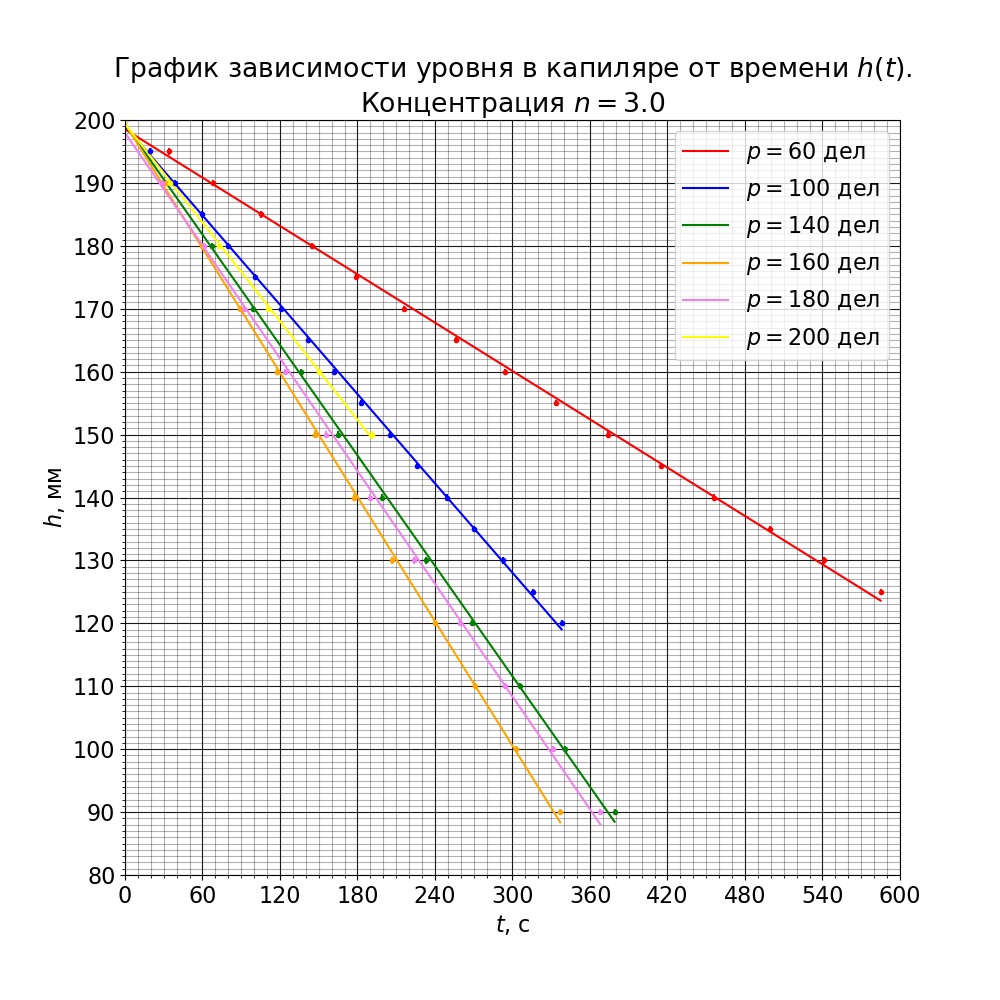
\includegraphics[width=1 \textwidth]{../plots/graph_h_t_0.png}
\end{figure}

Методом наименьших квадратов проведём наилучшую прямую $h~=~at~+~b$.

\begin{tabular}[t]{|c|c|c|c|c|}
\hline
$p$, дел & $a$, $\frac{мм}{с}$ & $\sigma_a$, $\frac{мм}{с}$ & $b$, мм & $\sigma_b$, мм \\ 
\hline
60 & -0,128 & 0,001 & 198,5 & 0,4 \\ 
100 & -0,237 & 0,001 & 199,0 & 0,3 \\ 
140 & -0,293 & 0,002 & 199,3 & 0,5 \\ 
160 & -0,329 & 0,003 & 199,4 & 0,5 \\ 
180 & -0,299 & 0,003 & 198,0 & 0,7 \\ 
200 & -0,261 & 0,003 & 199,4 & 0,4 \\ 
\hline
\end{tabular}

\begin{figure}[H]
	\centering
	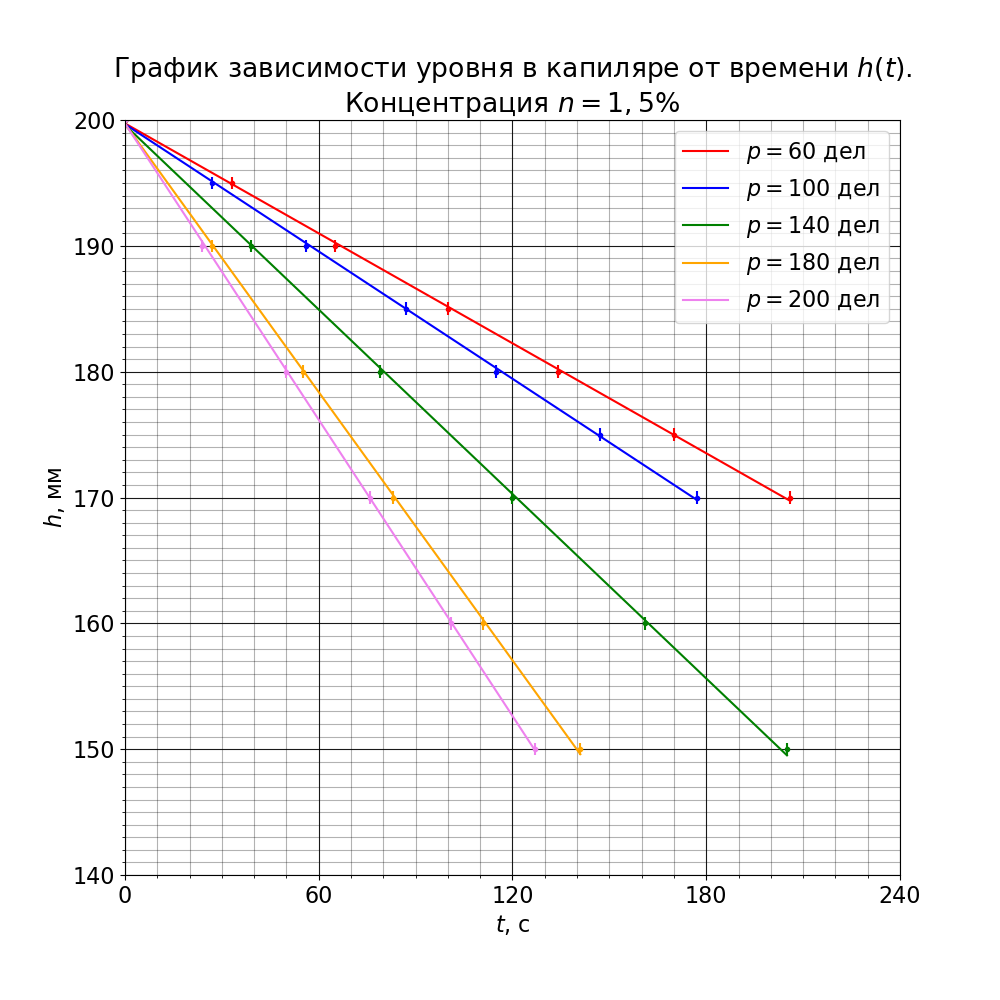
\includegraphics[width=1 \textwidth]{../plots/graph_h_t_1.png}
\end{figure}

Методом наименьших квадратов проведём наилучшую прямую $h~=~at~+~b$.

\begin{tabular}[t]{|c|c|c|c|c|}
\hline
$p$, дел & $a$, $\frac{мм}{с}$ & $\sigma_a$, $\frac{мм}{с}$ & $b$, мм & $\sigma_b$, мм \\ 
\hline
60 & -0,146 & 0,001 & 199,7 & 0,2 \\ 
100 & -0,169 & 0,002 & 199,7 & 0,2 \\ 
140 & -0,244 & 0,002 & 199,6 & 0,3 \\ 
180 & -0,355 & 0,003 & 199,7 & 0,2 \\ 
200 & -0,392 & 0,002 & 199,7 & 0,2 \\ 
\hline
\end{tabular}

\begin{figure}[H]
	\centering
	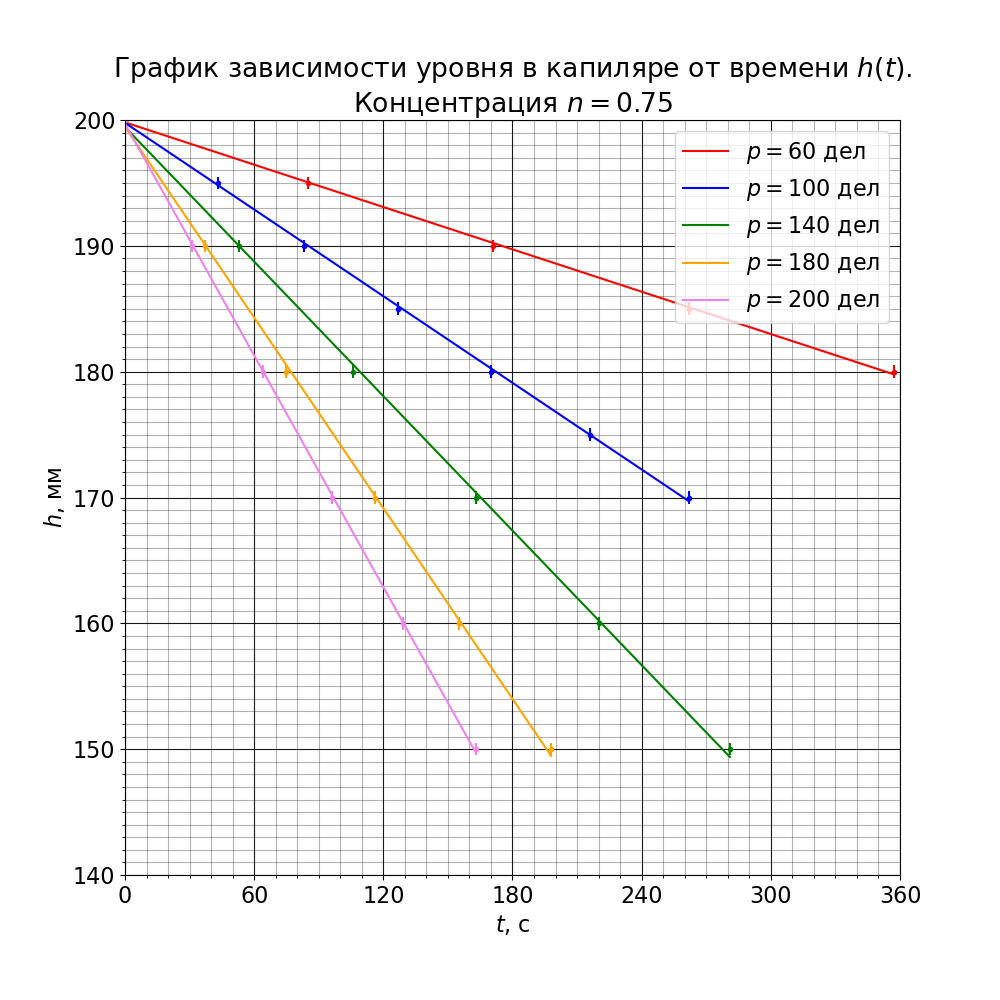
\includegraphics[width=1 \textwidth]{../plots/graph_h_t_2.png}
\end{figure}

Методом наименьших квадратов проведём наилучшую прямую $h~=~at~+~b$.

\begin{tabular}[t]{|c|c|c|c|c|}
\hline
$p$, дел & $a$, $\frac{мм}{с}$ & $\sigma_a$, $\frac{мм}{с}$ & $b$, мм & $\sigma_b$, мм \\ 
\hline
60 & -0,056 & 0,001 & 199,8 & 0,2 \\ 
100 & -0,115 & 0,001 & 199,8 & 0,2 \\ 
140 & -0,178 & 0,002 & 199,4 & 0,4 \\ 
180 & -0,253 & 0,003 & 199,5 & 0,4 \\ 
200 & -0,307 & 0,002 & 199,7 & 0,2 \\ 
\hline
\end{tabular}

\begin{figure}[H]
	\centering
	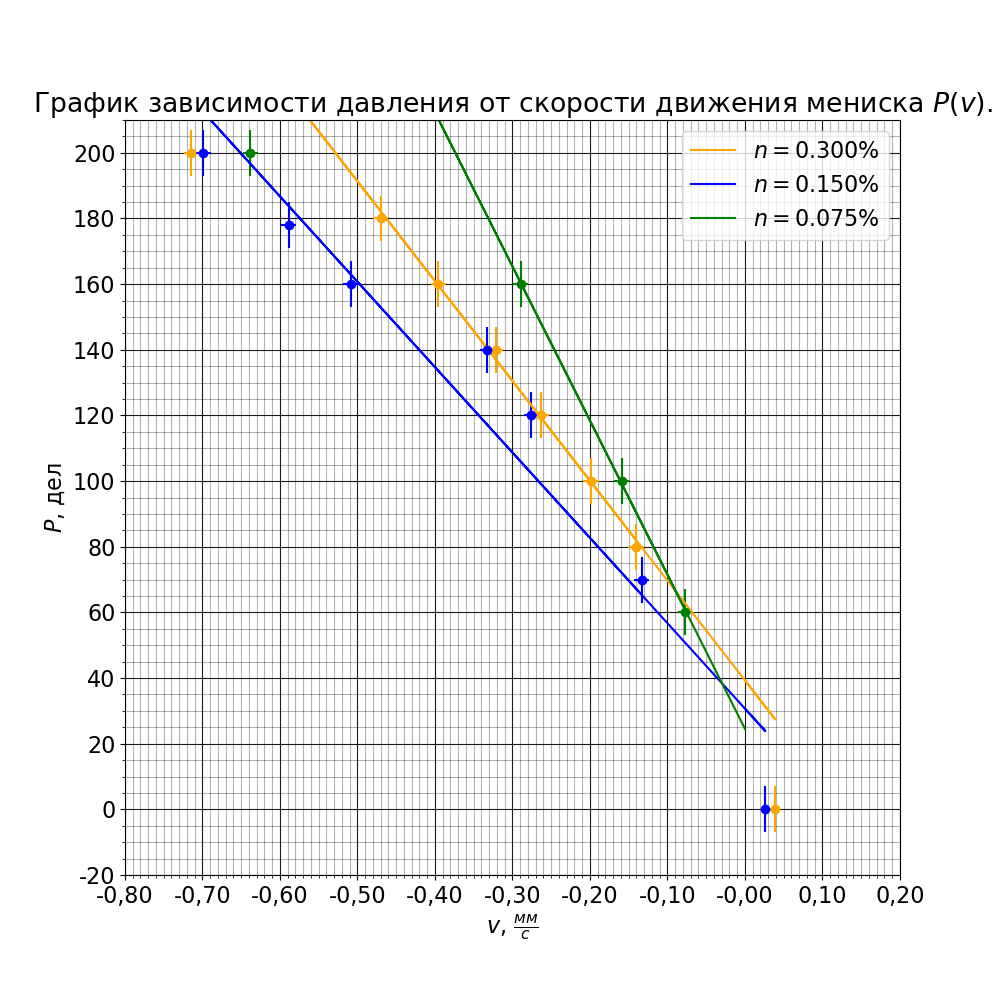
\includegraphics[width=1 \textwidth]{../plots/graph_v_p.png}
\end{figure}

Методом наименьших квадратов проведём наилучшую прямую $v~=~ap~+~b$.

\begin{tabular}[t]{|c|c|c|c|c|}
\hline
$n$, \% & $a$, $\frac{мм}{с \cdot дел}$ & $\sigma_a$, $\frac{мм}{с \cdot дел}$ & $b$, $\frac{мм}{с}$ & $\sigma_b$, $\frac{мм}{с}$ \\ 
\hline
<<<<<<< Updated upstream
3,00 & -0,0021 & 0,0004 & -0,0135 & 0,0400 \\ 
1,50 & -0,0019 & 0,0002 & -0,0064 & 0,0344 \\ 
0,75 & -0,0018 & 0,0001 & 0,0574 & 0,0144 \\ 
=======
0,30 & -0,0033 & 0,0001 & 0,1280 & 0,0114 \\ 
0,15 & -0,0036 & 0,0004 & 0,0908 & 0,0556 \\ 
0,08 & -0,0021 & 0,0000 & 0,0521 & 0,0041 \\ 
>>>>>>> Stashed changes
\hline
\end{tabular}

\begin{figure}[H]
	\centering
	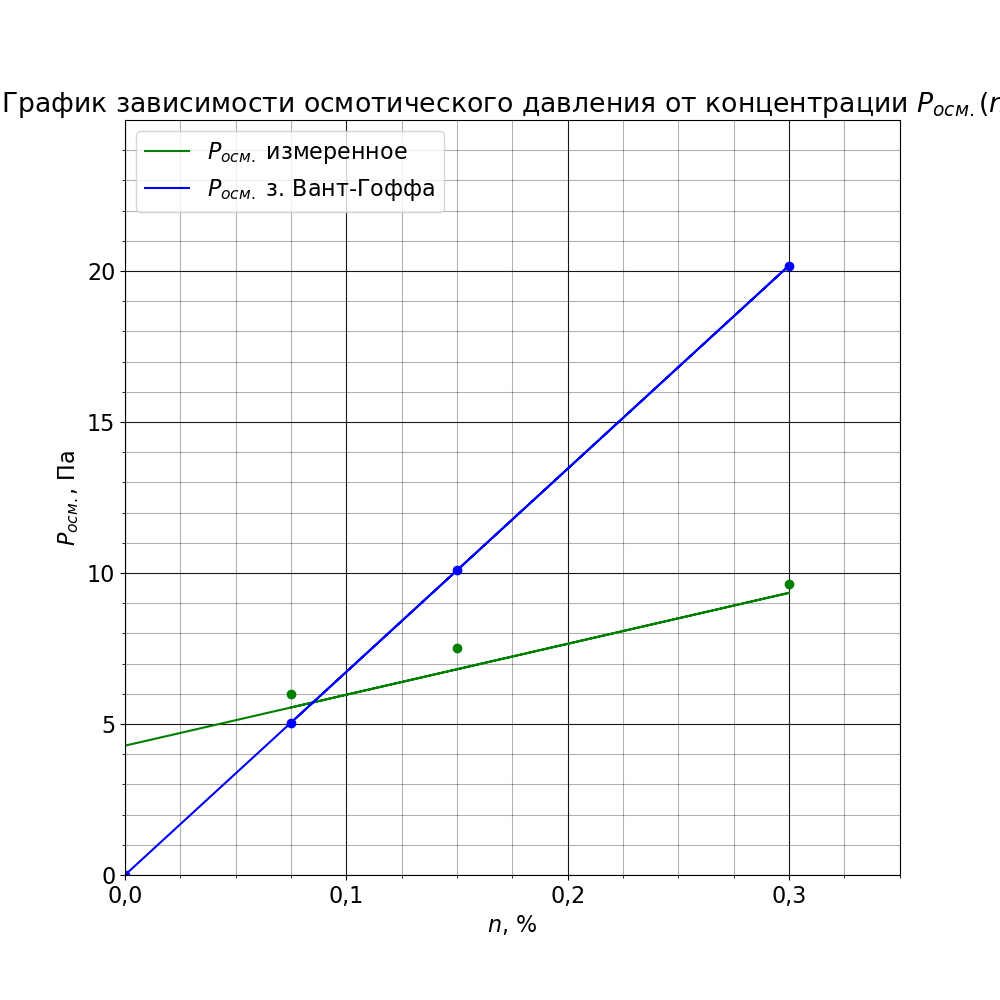
\includegraphics[width=1 \textwidth]{../plots/graph_p_osm_n.png}
\end{figure}

Методом наименьших квадратов по измеренных точкам проведём наилучшую прямую $P~=~an~+~b$. Также построим график зависимости осмотического давления от концентрации по закону Вант-Гоффа.

\begin{tabular}[t]{|c|c|c|c|}
\hline
$a$, $\frac{Па}{\%}$ & $\sigma_a$, $\frac{Па}{\%}$ & $b$, Па & $\sigma_b$, Па \\ 
\hline
16870,9881 & 5182,5088 & 4282,0069 & 1028,3722 \\ 
\hline
\end{tabular}
=======

\begin{figure}[H]
	\centering
	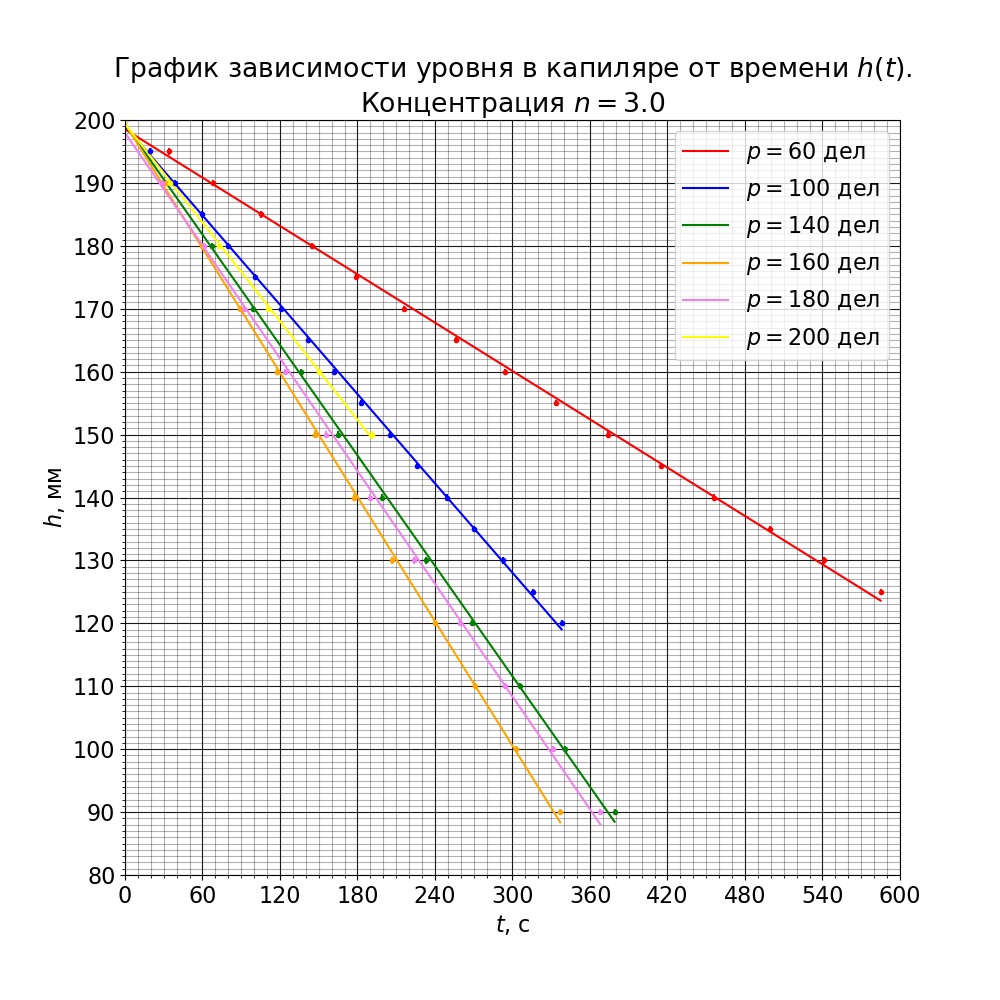
\includegraphics[width=1 \textwidth]{../plots/graph_h_t_0.png}
\end{figure}

Методом наименьших квадратов проведём наилучшую прямую $h~=~at~+~b$.

\begin{tabular}[t]{|c|c|c|c|c|}
\hline
$p$, дел & $a$, $\frac{мм}{с}$ & $\sigma_a$, $\frac{мм}{с}$ & $b$, мм & $\sigma_b$, мм \\ 
\hline
60 & -0,128 & 0,001 & 198,5 & 0,4 \\ 
100 & -0,237 & 0,001 & 199,0 & 0,3 \\ 
140 & -0,293 & 0,002 & 199,3 & 0,5 \\ 
160 & -0,329 & 0,003 & 199,4 & 0,5 \\ 
180 & -0,299 & 0,003 & 198,0 & 0,7 \\ 
200 & -0,261 & 0,003 & 199,4 & 0,4 \\ 
\hline
\end{tabular}

\begin{figure}[H]
	\centering
	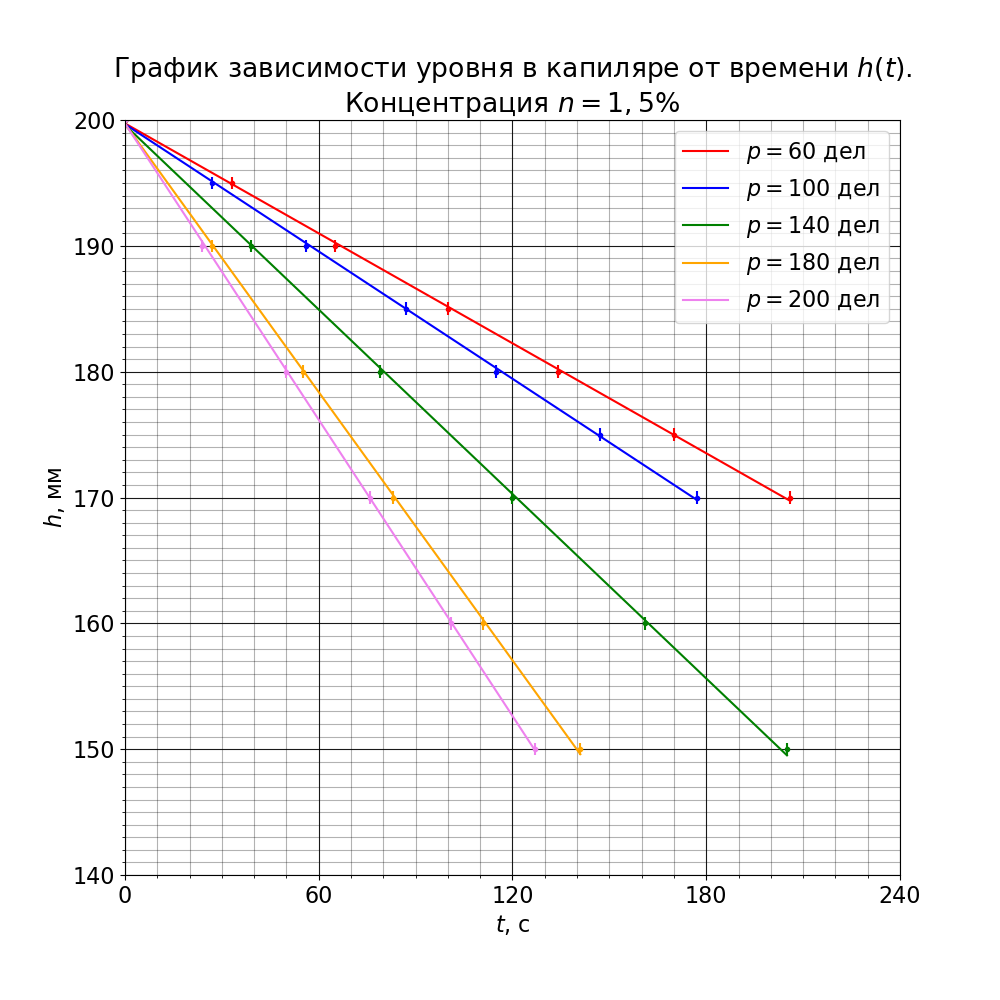
\includegraphics[width=1 \textwidth]{../plots/graph_h_t_1.png}
\end{figure}

Методом наименьших квадратов проведём наилучшую прямую $h~=~at~+~b$.

\begin{tabular}[t]{|c|c|c|c|c|}
\hline
$p$, дел & $a$, $\frac{мм}{с}$ & $\sigma_a$, $\frac{мм}{с}$ & $b$, мм & $\sigma_b$, мм \\ 
\hline
60 & -0,146 & 0,001 & 199,7 & 0,2 \\ 
100 & -0,169 & 0,002 & 199,7 & 0,2 \\ 
140 & -0,244 & 0,002 & 199,6 & 0,3 \\ 
180 & -0,355 & 0,003 & 199,7 & 0,2 \\ 
200 & -0,392 & 0,002 & 199,7 & 0,2 \\ 
\hline
\end{tabular}

\begin{figure}[H]
	\centering
	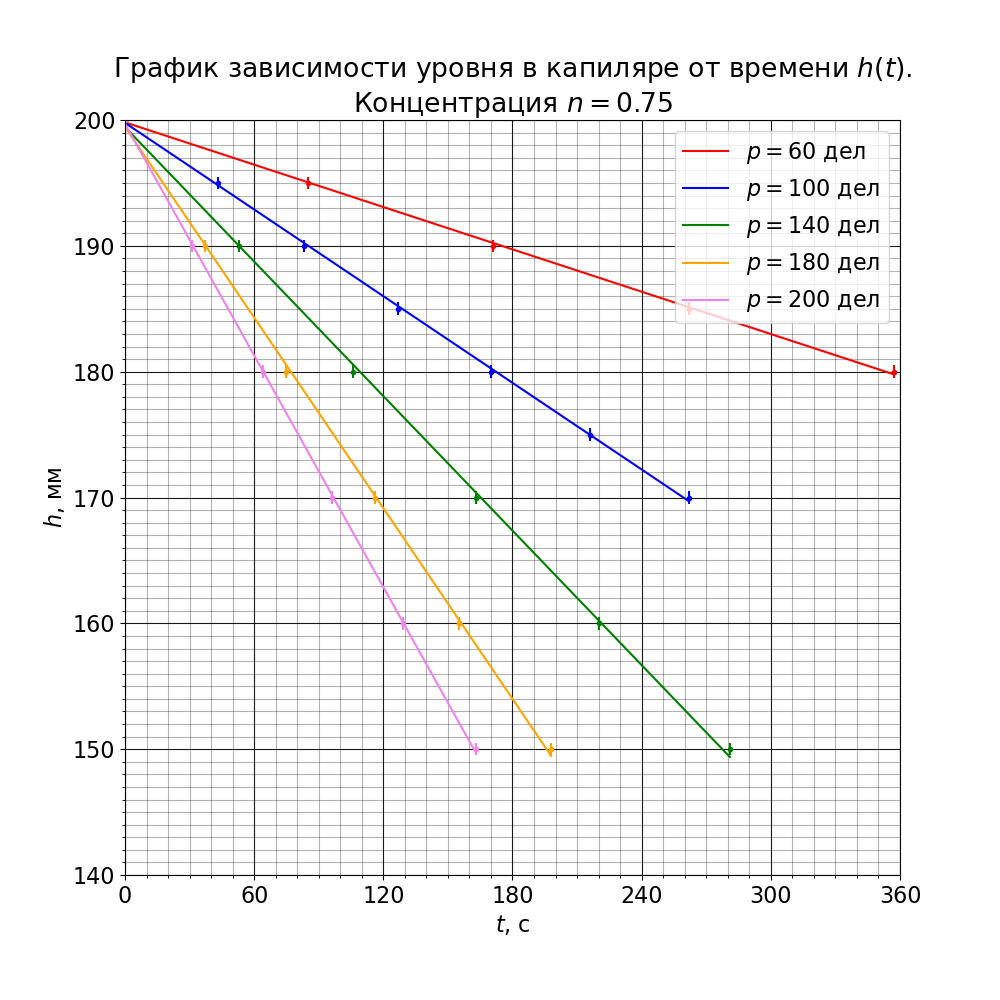
\includegraphics[width=1 \textwidth]{../plots/graph_h_t_2.png}
\end{figure}

Методом наименьших квадратов проведём наилучшую прямую $h~=~at~+~b$.

\begin{tabular}[t]{|c|c|c|c|c|}
\hline
$p$, дел & $a$, $\frac{мм}{с}$ & $\sigma_a$, $\frac{мм}{с}$ & $b$, мм & $\sigma_b$, мм \\ 
\hline
60 & -0,056 & 0,001 & 199,8 & 0,2 \\ 
100 & -0,115 & 0,001 & 199,8 & 0,2 \\ 
140 & -0,178 & 0,002 & 199,4 & 0,4 \\ 
180 & -0,253 & 0,003 & 199,5 & 0,4 \\ 
200 & -0,307 & 0,002 & 199,7 & 0,2 \\ 
\hline
\end{tabular}

\begin{figure}[H]
	\centering
	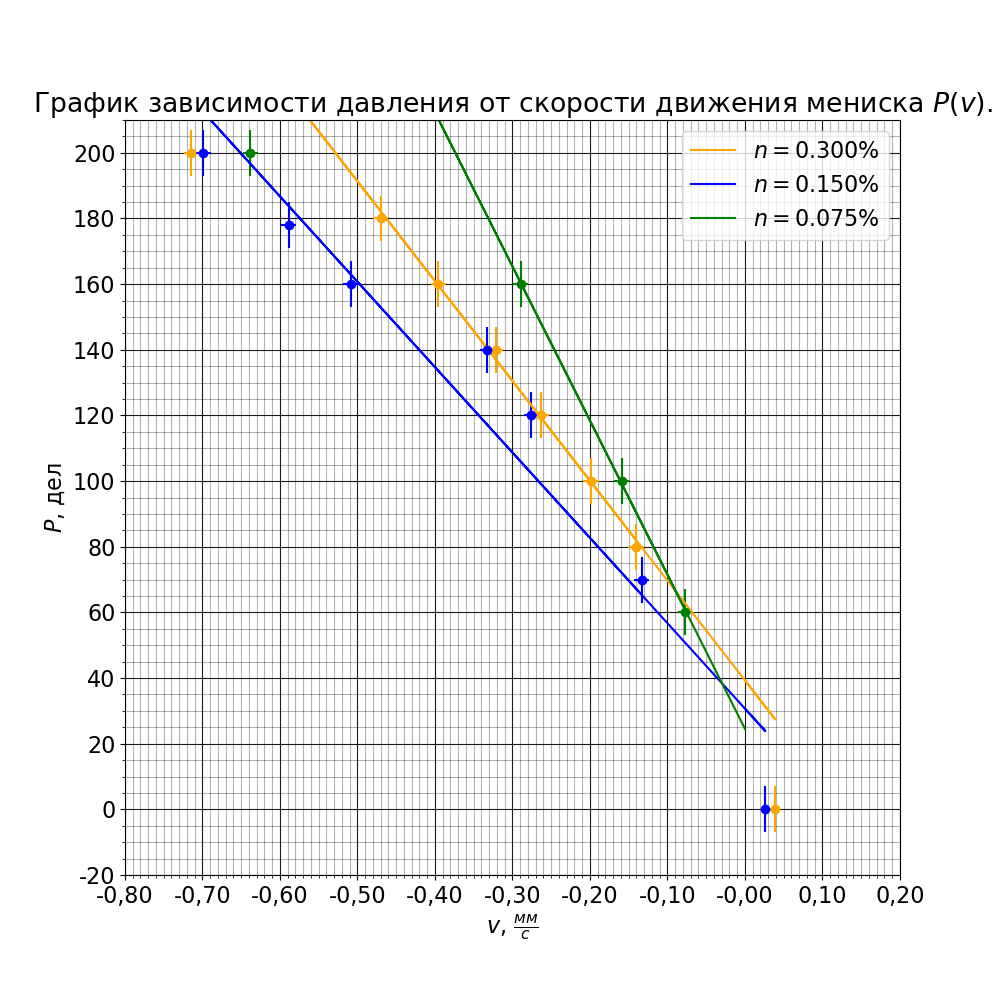
\includegraphics[width=1 \textwidth]{../plots/graph_v_p.png}
\end{figure}

Методом наименьших квадратов проведём наилучшую прямую $v~=~ap~+~b$.

\begin{tabular}[t]{|c|c|c|c|c|}
\hline
$n$, \% & $a$, $\frac{мм}{с \cdot дел}$ & $\sigma_a$, $\frac{мм}{с \cdot дел}$ & $b$, $\frac{мм}{с}$ & $\sigma_b$, $\frac{мм}{с}$ \\ 
\hline
<<<<<<< Updated upstream
3,00 & -0,0021 & 0,0004 & -0,0135 & 0,0400 \\ 
1,50 & -0,0019 & 0,0002 & -0,0064 & 0,0344 \\ 
0,75 & -0,0018 & 0,0001 & 0,0574 & 0,0144 \\ 
=======
0,30 & -0,0033 & 0,0001 & 0,1280 & 0,0114 \\ 
0,15 & -0,0036 & 0,0004 & 0,0908 & 0,0556 \\ 
0,08 & -0,0021 & 0,0000 & 0,0521 & 0,0041 \\ 
>>>>>>> Stashed changes
\hline
\end{tabular}

\begin{figure}[H]
	\centering
	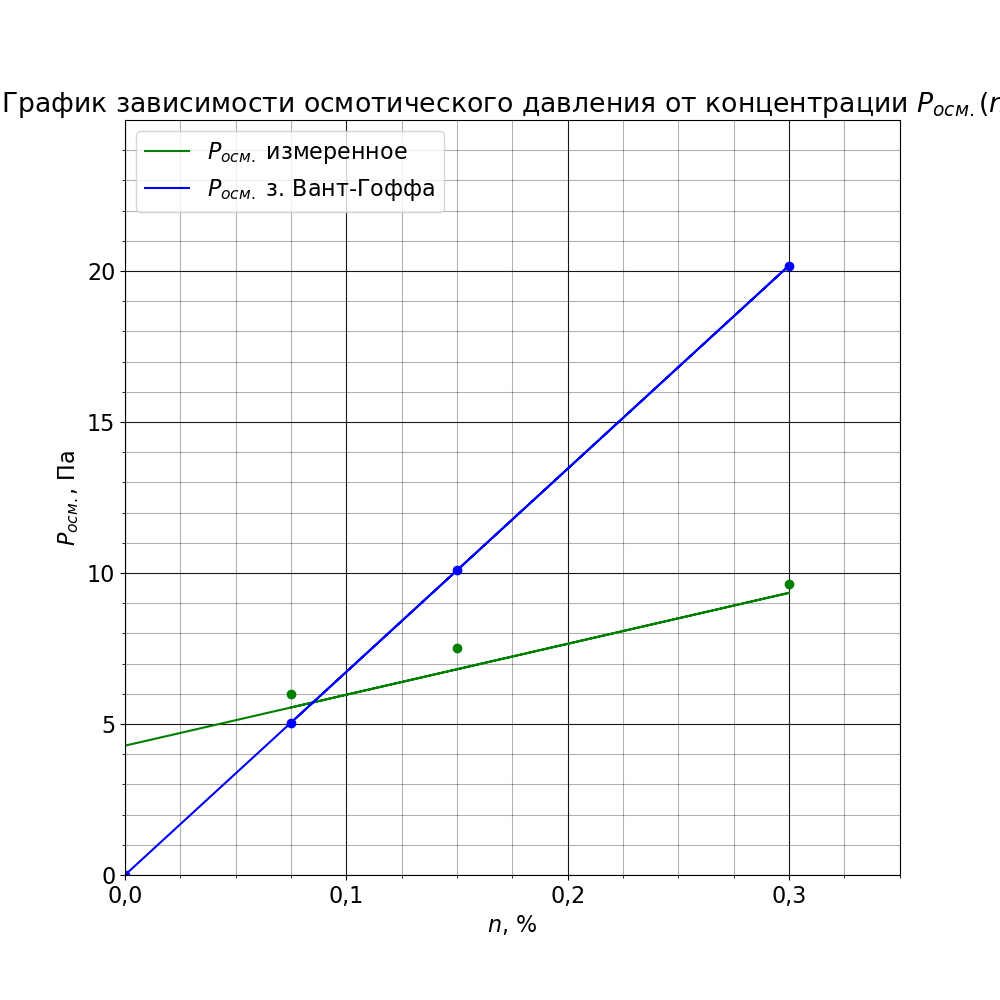
\includegraphics[width=1 \textwidth]{../plots/graph_p_osm_n.png}
\end{figure}

Методом наименьших квадратов по измеренных точкам проведём наилучшую прямую $P~=~an~+~b$. Также построим график зависимости осмотического давления от концентрации по закону Вант-Гоффа.

\begin{tabular}[t]{|c|c|c|c|}
\hline
$a$, $\frac{Па}{\%}$ & $\sigma_a$, $\frac{Па}{\%}$ & $b$, Па & $\sigma_b$, Па \\ 
\hline
16870,9881 & 5182,5088 & 4282,0069 & 1028,3722 \\ 
\hline
\end{tabular}
>>>>>>> Stashed changes
>>>>>>> Stashed changes
